\documentclass{article}
\usepackage{graphicx}
\usepackage{multicol} % use to multiple column in itemize
\usepackage{float}
\usepackage{setspace}
\usepackage{hyperref}
\setlength{\parskip}{0.5em}

\begin{document}

\title{Regression}
% \author{Cong Cuong PHAM}

\maketitle

\begin{abstract}
This document introduces some fundamental notions of Regression.
\end{abstract}

\subsection{Regression (Supdervised)}
\par The goal of regression is to predict a continuous-valued feature associated with a sample. Continuous-valued meaning small changes in the input result in small changes in the output.

Imagine hiking from Portland, OR to Seattle, WA. As time progresses, your distance from Portland increases and your distance to Seattle decreases. Even though you stop for meals and to rest, these distance values transition smoothly. Throughout the course of your hiking, you never magically {\it{teleport}} a large distance. Instead, you smoothly and incrementally make your way step-by-step. With regression, a mathematical relationship is modeled for your samples so that as you gently alter one feature, another feature responds by being altered as well.

\begin{figure}[H]
\centering
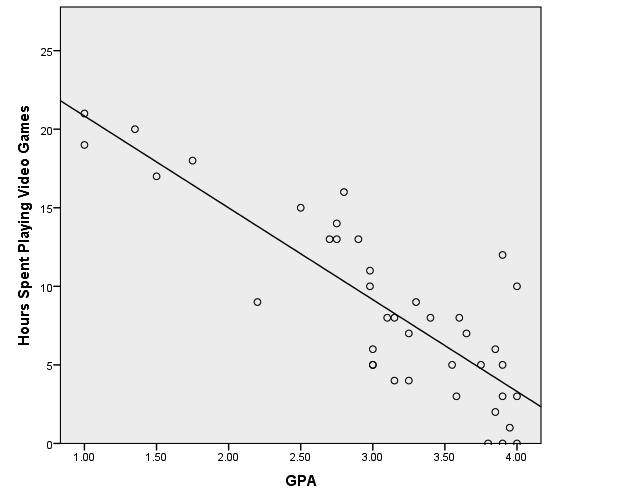
\includegraphics[width=0.6\linewidth]{pic/regression.png}
\caption{Example of linear regression.}
\end{figure}

More examples

\begin{itemize}
    \item Calculate an equation to predict the size of a house given its price; or the price of a house given its size.
    \item Explore if a correlation exists between hours a student spends studying, spends watching TV, and their final exam score.
    \item Estimate how many power plants should be constructed in the next 50 years, based upon the historical energy consumption per household.
    \item Figure out how many days a person has left to live based on the severity of their symptoms.
\end{itemize}

\par Regression falls into the realm of supervised learning because in order for it to work, you have to provide the computer with labeled samples. It then attempts to fit an equation to the samples' features.

\begin{flushright}
    source: \href{https://courses.edx.org/courses/course-v1:Microsoft+DAT210x+6T2016/courseware/e36e6b45ae5d4032bef2ec557c1ff48f/a8cf8333f6044e9b9a357b7797f282e3/?child=first}{course.edx.org}  
\end{flushright}
\end{document}